% Experimental Setup draft. Generated by make_paper_text.py -- do not edit numbers by hand.
\section{Experimental setup}
\label{sec:setup}

\subsection{Data and splits}
\label{sec:setup-data}

We use the validation splits of DocVQA~\cite{docvqa} (5,349 questions over 1,286 page images) and
InfographicVQA~\cite{infovqa} (2,801 questions over 500 infographics), taken from the Hugging Face copy
\texttt{lmms-lab-encoder/DocVQA} at revision \texttt{539088e} (Table~\ref{tab:data}); the public test splits have no answers. We use
all 8,150 questions of both validation sets (66\% DocVQA), without subsampling or balancing. Page images
are stored at their original resolution (median 3.8 megapixels); ColPali encodes each page at
448$\times$448 pixels and the generator receives at most 1280 visual tokens (about 1.0 megapixels). Each
dataset's pages form its own retrieval pool.

Routers are trained and evaluated on 5 splits (seeds 1234--1238). Each split assigns whole
pages to training, validation and test (60/20/20 within each dataset), so all questions about a page (4.6 on
average) fall in the same split; test splits hold 1,548--1,653 questions. Splits group by page, not by
document: 129 of the 178 multi-page DocVQA documents have pages in more than one split (seed
1234). Training data are used to fit the routers; validation data are used for early stopping, hyperparameter
selection, the choice of $\lambda$ and the calibration of escalation probabilities. No parameter of the final pipeline
is fitted or selected on test data. However, the router design itself (Section~\ref{sec:method-routers}) was developed
on the same five splits, and the feasibility analyses that motivated it inspected their test portions; no separate
confirmation set was held back (Section~\ref{sec:res-limits}).

\begin{table}[t]
\centering
\caption{Evaluation data (validation splits). Natural = all questions; stratified = up to 150 per (dataset, question type). docTR OCR of all pages: 471\,s, 29.3\,kJ on one RTX 4090.}
\label{tab:data}
\begin{tabular}{lrrr}
\toprule
\textbf{Dataset} & \textbf{Questions} & \textbf{Pages} & \textbf{Stratified} \\
\midrule
docvqa & 5349 & 1286 & 1014 \\
infovqa & 2801 & 500 & 830 \\
Total & 8150 & 1786 & 1844 \\
\bottomrule
\end{tabular}
\end{table}


\subsection{OCR and retrieval}
\label{sec:setup-retrieval}

OCR is run once on every page with docTR~\cite{doctr} (DBNet-ResNet50 detection and CRNN-VGG16 recognition) on the GPU.
Pages more than twice as tall as they are wide are split into vertical tiles of 1.5 times their width so that the
detector's resizing does not shrink the text; this applies to 276 of the 500 infographics and
14 DocVQA pages (at most 8 tiles). OCR of all 1,786 pages took 471\,s; no page
produced empty text.
\emph{Text retrieval} uses BM25 (Okapi; rank-bm25 with $k_1 = 1.5$, $b = 0.75$, $\epsilon = 0.25$) over lower-cased ASCII
alphanumeric tokens of the OCR text.
\emph{Visual retrieval} uses ColPali v1.3~\cite{colpali} (revision \texttt{b5c6dd6}; PaliGemma-3B base,
revision \texttt{30ab955}) in bf16. Each page is encoded once into 1031 vectors of dimension 128 (1,024 patch
vectors and the prompt tokens), and queries are scored by exhaustive MaxSim against all pages of the pool on the GPU.
Retrieval quality is reported in Table~\ref{tab:retrieval}.

\begin{table}[t]
\centering
\caption{Page retrieval over each dataset's page pool. ColPali per query: encode 46\,ms + score 1.1\,ms (p50); index build 210\,s for 1786 pages, 450\,MB.}
\label{tab:retrieval}
\begin{tabular}{lrrrrr}
\toprule
\textbf{Retriever} & \textbf{R@1} & \textbf{R@3} & \textbf{R@5} & \textbf{R@10} & \textbf{MRR} \\
\midrule
BM25 (docTR text) & 0.439 & 0.546 & 0.586 & 0.633 & 0.507 \\
ColPali v1.3 & 0.573 & 0.697 & 0.749 & 0.798 & 0.651 \\
\bottomrule
\end{tabular}
\end{table}


\subsection{Generation}
\label{sec:setup-generation}

All paths use Qwen2.5-VL-7B-Instruct~\cite{qwen25vl} (revision \texttt{cc59489}) in bf16 with scaled dot-product attention (SDPA), greedy
decoding, at most 32 new tokens and the model's default repetition penalty (1.05). The system prompt is
the same for every path: ``You answer questions about documents. Reply with only the answer: a short phrase, number or name, copied exactly from the document when possible. No explanation.'' The user turn contains, in this order, the page image (visual and
hybrid paths), the text context as ``Document text:'' followed by ``[Page $i$ OCR]'' blocks (text and hybrid paths),
and ``Question: $q$ / Answer:''. The text context is the first 2,000 characters of each of the top 3
BM25 pages. Page images are resized with the model's own resizing rule to between 256 and
1280 visual tokens.

The GPU also drives the Windows desktop under the Windows Display Driver Model (WDDM). When its memory is exhausted, the NVIDIA driver's system-memory
fallback silently moves allocations to host RAM, which slows execution by an order of magnitude instead of failing.
The token and character caps were chosen to keep peak reserved memory below this point; in the main run the peak was
22.9\,GiB, 7 hybrid queries exceeded 21\,GiB, and no generation took longer than
2.1\,s, so no measurement was affected.

\subsection{Measurement protocol}
\label{sec:setup-measurement}

Each path is run once on every query, one query at a time (batch size 1), with no other compute job on the GPU. Models
are warmed up before timing; timed regions are bracketed by CUDA synchronisation. Cached GPU memory is released before
each generation, outside the timed region; this means the generation timing includes re-allocating that memory, which
a long-running server would avoid. Retrieval was timed in separate passes: BM25 on the CPU, and ColPali query encoding
and scoring on the GPU (one value per query, shared by the visual and hybrid paths). Per query and path we record:
wall-clock time of preprocessing, retrieval and generation; GPU-seconds, i.e.\ the wall-clock time of the GPU stages
(generation, plus ColPali for paths that use it), including host overhead such as tokenisation; energy as the
difference of the NVML total-energy counter (millijoule resolution; values for single short queries are approximate,
totals are accurate); peak allocated and reserved GPU memory; and the generated answer with the mean and minimum
log-probability of its tokens under the raw logits. Offline costs (OCR and ColPali indexing) are measured separately
and are not included in per-query costs.

Router overhead is measured on its own. For CAVR (mpnet embedding in fp16 and the MLP on the GPU), latency is the
median over 500 single queries and throughput is measured at batch sizes up to 1,024. For CAVR-CE
(embedding, passage selection, tokenisation and the cross-encoder), latency is the median over 300 single
queries; throughput of the cross-encoder forward pass is measured at batch sizes up to 256. Timing does
not depend on the weights, so both benchmarks use untrained heads.

\subsection{Metrics}
\label{sec:setup-metrics}

Answer quality is measured with ANLS~\cite{anls}: the normalised Levenshtein similarity to the closest reference
answer, set to zero below 0.5. Before comparison, answers are converted to the Unicode normal form NFKC, lower-cased, whitespace is collapsed,
and leading and trailing spaces, periods, commas, colons, semicolons and quotation marks are stripped. This differs
from the official evaluation, which only lower-cases and strips whitespace, by at most 0.0003 ANLS on any path.
Exact match uses the same normalisation. A router's \emph{success AUC} is the area under the ROC curve of its predicted
quality for the event ANLS $\ge$ 0.5, computed per path on test and averaged over the three paths. Cost is measured in
GPU-seconds and joules per query, and latency as p50 and p95 wall-clock time.

\subsection{Policies compared}
\label{sec:setup-policies}

\begin{itemize}
  \item \emph{Fixed policies:} always-text, always-visual and always-hybrid.
  \item \emph{Keyword rule:} a hand-written rule that routes by keywords in the question, applied as written (its
  patterns matched as plain substrings) and with its patterns applied as regular expressions.
  \item \emph{Random at equal budget:} paths drawn independently with CAVR's path mix (200 draws), and a
  quality-blind mix of always-visual and always-hybrid at CAVR-CE's GPU cost, evaluated in expectation per seed.
  \item \emph{Logistic regression:} one classifier per $\lambda$ on the question embedding, predicting the outcome
  label; regularisation $C \in \{0.1, 1, 10\}$ chosen on validation utility.
  \item \emph{$k$-nearest neighbours (kNN):} regression of per-path ANLS from the $k$ nearest training questions (cosine distance,
  $k \in \{5, 10, 25, 50, 100\}$ chosen on validation utility at $\lambda = 0.1$), followed by the decision rule of
  Section~\ref{sec:method-formulation}.
  \item \emph{CAVR}, its class head used alone (``CAVR (class head only)''), and two ablations that add BM25 scores, or
  BM25 and ColPali scores, to its input.
  \item \emph{CAVR-CE}, the content-aware router (Section~\ref{sec:method-routers}), and a gradient-boosting baseline on
  the same tabular features without the cross-encoder or the ColPali token statistics (histogram gradient boosting,
  300 iterations, learning rate 0.05, 31 leaves).
  \item \emph{Per-query oracle:} the path that maximises measured ANLS minus $\lambda$ times measured per-query cost.
\end{itemize}
Unless stated otherwise, routers use $\lambda = 0.1$, and $\lambda$ sweeps use \{0, 0.02, 0.05, 0.1, 0.2, 0.3, 0.5, 1\}. For the operating
point of CAVR-CE, $\lambda$ is chosen on each split's validation set from \{0, 0.005, 0.01, 0.02, 0.03, 0.05, 0.075, 0.1, 0.15, 0.2, 0.3, 0.5, 0.75, 1, 1.5, 2\} as the cheapest value whose
validation ANLS is within 0.005 of always-hybrid; on split 3 no value reaches this target, and the
$\lambda$ with the highest validation ANLS (0.01) is used.

\paragraph{Training behaviour.} Figure~\ref{fig:training} shows training and validation losses, re-recorded by
re-training both routers with the same settings and seeds (the CAVR runs reproduce the original epoch counts and
validation utility exactly; CAVR-CE validation AUC differs by at most 0.003). Both routers overfit quickly on
about 4,900 training questions. CAVR's training loss keeps falling while its validation loss reaches its minimum
after a few epochs; early stopping on validation utility keeps epochs 4--9. For CAVR-CE,
validation cross-entropy is lowest after the first epoch (0.484) and rises to 0.617 by epoch
5, while validation AUC peaks at epoch 2 (0.846); the epoch with the best validation AUC is
kept, which is epoch 2 on 5 of 5 splits.

\begin{figure*}[t]
  \centering
  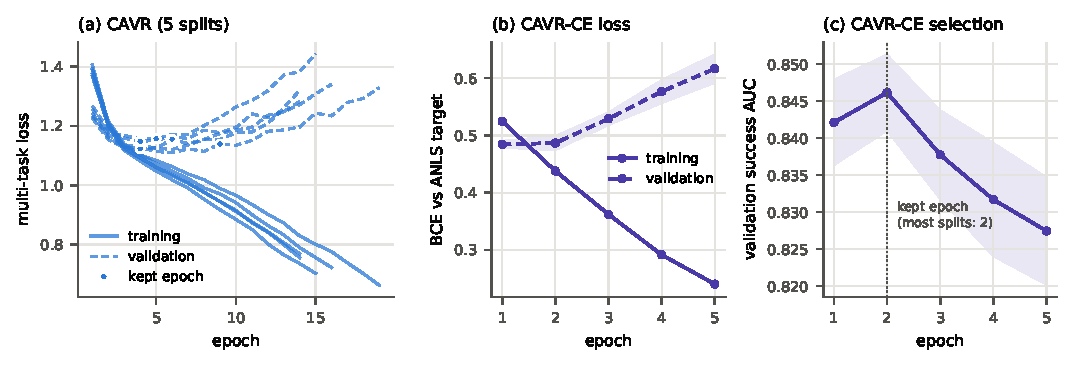
\includegraphics[width=\textwidth]{figures/training_curves.pdf}
  \caption{Training and validation curves. (a) CAVR multi-task loss on each split (training solid, validation dashed);
  dots mark the epoch whose weights are kept (best validation utility). (b) CAVR-CE binary cross-entropy against ANLS
  targets and (c) its validation success AUC, mean $\pm$ standard deviation over splits; the dotted line marks the kept
  epoch.}
  \label{fig:training}
\end{figure*}

\paragraph{Retrieval-depth and gold-page controls.} On a seeded sample of 750 questions per dataset, the
generator is run with the same prompt, caps and decoding on five further contexts: the top-1 BM25 page as text, the
top-3 ColPali page images, and the gold page as text, as an image, and as both. These runs were made on the
NVIDIA A10 node; to check that it reproduces the workstation, the main text and visual paths were re-run there on
200 of the questions, and the hybrid path on the same questions, giving identical answers for
98.5\%, 97.5\% and 97.5\% of them (ANLS 0.522 against 0.516 for the
visual path and 0.502 against 0.509 for the hybrid path). Differences are paired per question with page-cluster bootstrap
intervals.

\subsection{Held-out confirmation set}
\label{sec:setup-confirm}

After the design was fixed, a confirmation set was drawn from the training splits of the same Hugging Face copy
(revision \texttt{539088ef8a8a}): a seeded sample of 750 questions per dataset from 6 training-split
files, whose 1,662 DocVQA pages and 791 infographics form the retrieval pools. No page is shared
with the validation data. OCR, BM25 and ColPali retrieval, generation on all three paths and the CAVR-CE features were
run with the unchanged pipeline on the NVIDIA A10 node. One question was excluded because its hybrid input
(5,184 tokens) did not fit in that GPU's memory. CAVR-CE was re-trained for each seed on that seed's original
training split, the confirmation features were standardised with the same split's statistics, and the decision rule,
$\lambda$ and cost estimates were not changed. Comparisons use the paired page-cluster bootstrap and McNemar tests
described next.

\subsection{Statistical analysis}
\label{sec:setup-stats}

Policy results are means and sample standard deviations over the 5 splits; the splits overlap, so these
standard deviations describe split-to-split variation rather than independent replications. Within a split, two
policies are compared on the same test queries with McNemar's exact test on exact match, and with a paired bootstrap
of the ANLS difference that resamples whole pages (1000 resamples, 95\% percentile intervals), because questions
about the same page are not independent. McNemar's test treats questions as independent and is therefore somewhat
liberal. The five test splits together cover 5,419 of the 8,150 questions; 2,150 are tested more than
once and 2,731 never. Counts across splits, such as the number of splits on which a difference is
significant, are therefore descriptive, and the policy comparisons are exploratory and not corrected for multiple
testing. Calibration is measured by the expected calibration error with ten equal-width bins.

\subsection{Serving and scaling experiments}
\label{sec:setup-serving}

\paragraph{Batched generation.} Each path is run on 32 questions drawn from a stratified sample (up to 150
questions per dataset and question type) at batch sizes 1, 2, 4, 8 and 16 (hybrid: up to 8). Batch sizes whose peak
reserved memory exceeded 21\,GiB (within 3\,GiB of the GPU's memory) are excluded, which leaves a largest batch of 8 for the text
and visual paths and 4 for the hybrid path; batch sizes in between are interpolated linearly.

\paragraph{Load test.} A discrete-event simulation serves Poisson arrivals with a pool of identical GPUs and an ideal
global queue. Requests are drawn with replacement from a split's test queries. A free GPU takes the oldest waiting
request and batches it with the other waiting requests of the same path, without waiting for more; a batch takes the
mean measured generation time of its members, scaled by the measured batching curve, plus the sum of their ColPali
times. CPU-side work adds latency only (unlimited CPU). Each point is one simulation of 6,000 requests with a fixed
random seed; the first 500 are discarded. Single-GPU capacity is the highest rate on a grid of
0.25\,queries/s steps from 0.25 to 6 and coarser steps up to 20, at which p95 latency stays
within 2\,s; a value of 0 means below 0.25\,queries/s. The number of GPUs needed for a load of 5, 10, 25, 50 and 100
queries/s is the smallest pool, up to 256 GPUs, that holds p95 within the target, found by doubling and then binary
search. Results at p95 $\le$ 2\,s are averaged over the 5 splits; the 5\,s sensitivity check, the latency
curves and the $\lambda$ operating points use split 1.

\paragraph{Live serving.} To check the simulator, the generation stage was also served live on the node with two
NVIDIA A10 GPUs (Table~\ref{tab:hardware_multigpu}). vLLM 0.31.0~\cite{vllm} (PyTorch 2.13.0) runs in
Ubuntu 24.04 under version 2 of the Windows Subsystem for Linux (WSL), with the GPUs in the Microsoft Compute Driver Model
(MCDM), the Windows driver mode that gives WSL access to a GPU without a display. Each GPU holds one replica of
Qwen2.5-VL-7B in bf16 with the same model revision, image-size limits and greedy decoding as the cached run, at most 16
concurrent sequences and prefix caching off. FlashInfer's sampler is disabled because it compiles at start-up with a
CUDA toolkit that the WSL image lacks; under greedy decoding this does not change the tokens. Retrieval and routing
ran beforehand, so only generation is served: the client sends each query's prompt as built for the cached run and
dispatches it to the replica with the fewest outstanding requests. A pilot of 50 requests per path
checked the prompts against the workstation run. Service times were measured one request at a time on all
1,606 split-1 test queries for every path, and the batching curve as the latency ratio at 1 to 16 concurrent
requests. The load test sends open-loop Poisson arrivals (fixed seed) at 15--110\% of the replicas' measured peak
throughput for the policy's path mix, with at most 400 arrivals per rate, the first 10\% discarded, and stops once p95
exceeds 30\,s. Each measured arrival trace is then replayed through the simulator above, once with the A10's service
times and batching curve and once with the workstation's, so that predicted and measured p95 refer to the same
arrivals; the capacity at a p95 target is interpolated between tested rates.

\paragraph{Sensitivity and control experiments.} With the same simulator, the GPUs needed for 100 queries/s are
found for p95 targets of 1.5, 2, 3, 5, 7.5 and 10\,s on all five splits for always-visual, always-hybrid and
CAVR-CE; the 2 and 5\,s targets are repeated with each batch charged its longest member's generation time. For a
large corpus, a retrieval tier is added by projection: ColPali GPU-seconds per query at batch 64 on the workstation,
measured at the largest GPU-resident size and scaled linearly in pages, times the share of queries that need
ColPali, at full utilisation, and at least as many GPUs as are needed to hold the index. Load-adaptive $\lambda$ is
simulated on split 1 with a fixed pool under alternating Poisson rates; the controller moves one step up the
$\lambda$ sweep each time the waiting time of the oldest queued request doubles past a base threshold, which is
chosen on the split's validation queries (the highest ANLS with at least 95\% of requests within 2\,s, else the
highest share within 2\,s).

\paragraph{Index scaling.} Corpora of 1k, 10k, 50k and 100k pages are built by repeating the real page embeddings. We time
exhaustive MaxSim with the index resident on the GPU (when it fits within 18\,GiB), streamed in chunks from
pinned host memory, pooled 2$\times$2 over the patch grid (1,024 patch vectors to 256, re-normalised, plus the 7 prompt
tokens: 263 vectors), and split into shards that each fit one GPU. Hierarchical token pooling, following
Clavi\'e et al.~\cite{tokenpooling}, clusters each page's
1,024 patch vectors by Ward linkage into 1,024/$f$ clusters ($f = 2, 3, 4$), averages and re-normalises each cluster
and keeps the prompt-token vectors; recall@1 and recall@5 of the gold page are measured for all questions over each
dataset's page pool with the same batched query embeddings for every variant. On this workstation sharding is emulated by timing
the shards one after another and reporting the slowest shard, without the cost of merging results; it is measured on
real GPUs below. Latency is the median
over 50 single queries (all from DocVQA); throughput uses query batches of 1, 4, 16, 64 (streamed index: 1, 4
and 16), with at least two repetitions per batch size.

\paragraph{Multi-GPU sharding.} Sharding is measured on two further machines, one with three Tesla P40 GPUs and one with
two NVIDIA A10 GPUs, all in Tesla Compute Cluster (TCC) mode, NVIDIA's compute-only driver model (Table~\ref{tab:hardware_multigpu}), with the same benchmark script. The page embeddings of the evaluation corpus and the per-token embeddings of
the questions are exported from the workstation, so no model runs on these nodes. A corpus of 1k to 150k pages,
built by repeating the real pages (page $j$ is real page $j$ modulo the 1,786 evaluation pages), is split into one
contiguous shard per GPU, stored in fp16 and scored by exhaustive MaxSim in fp32 on the Tesla P40, whose fp16 arithmetic is slow, and
in fp16 on the NVIDIA A10. Each query is sent to all shards at
once, one host thread per GPU; each shard returns its top-10 pages and the host merges them, so the measured
latency includes dispatch and merge. Shards larger than 70\% of GPU memory (15.7\,GiB on the Tesla P40,
15.6\,GiB on the NVIDIA A10) are not run. Before timing, the sharded top-1 page on the real corpus is compared with one GPU for 500 questions.
Latency is the median and 95th percentile over 50 single queries; throughput and energy use query batches of
1, 4, 16 and 64. Energy is read from the NVML counters of all GPUs of the node, so runs on fewer GPUs include the idle
draw of the unused ones, which we estimate from the runs themselves (Section~\ref{sec:res-scale}).

\paragraph{Index in host memory.} On the NVIDIA A10 node, corpora of 100k, 250k, 500k and 1M pages, built in the same way, are held
in host memory (up to 246\,GiB) and streamed to the GPUs for every query batch. Windows refuses page-locked
(pinned) allocations of this size, so the index is allocated as ordinary memory and then page-locked with
\texttt{cudaHostRegister} in blocks of 16\,GiB. With $g$ GPUs the corpus is split into $g$ contiguous
shards. For each batch, every GPU copies its shard over PCIe in chunks of 4,068 pages
(1.0\,GiB) into two device buffers, so that copying one chunk overlaps scoring the other; no copy spans
two registered blocks. Scoring is exhaustive MaxSim in fp16, as in the GPU-resident runs on this node; each GPU keeps
its top-10 pages and the host merges them. Before timing, the top-1 page (up to the repetition of real pages) and score
of streamed search are compared with GPU-resident search, sharded over both GPUs, for 100 questions on 100k pages.
Latency is the median over 5 single queries after one warm-up pass; throughput and energy use batches of
1, 16 and 64 with 2 repetitions each. The PCIe copy rate alone is measured by streaming the largest index
without scoring. Energy is the sum of the NVML counters of both GPUs.

\subsection{Hardware, software and reproducibility}
\label{sec:setup-hardware}

All experiments except multi-GPU sharding and the host-memory index ran on the workstation of
Table~\ref{tab:hardware}, which also lists the library versions and model revisions; these two ran on the nodes of
Table~\ref{tab:hardware_multigpu}. Seeds are fixed (1234 for data sampling and the first split). The CAVR MLP is trained on the
CPU and is deterministic; generation, ColPali and CAVR-CE fine-tuning run on the GPU in bf16 and are reproducible up to
small numerical differences (re-training CAVR-CE changed validation AUC by at most 0.003). Every query's
outputs are cached, every table and figure in this paper is generated from the cached results by the released code
[AUTHOR ACTION: cite the release and its DOI], and the hash of the generation script is stored with its outputs.

\begin{table}[t]
\centering
\caption{Workstation used for every measurement except multi-GPU index sharding (Table~\ref{tab:hardware_multigpu}): hardware, software and model revisions.}
\label{tab:hardware}
\begin{tabular}{ll}
\toprule
\textbf{Component} & \textbf{Value} \\
\midrule
GPU & 1 $\times$ NVIDIA GeForce RTX 4090 (24\,GiB, power limit 450\,W) \\
Driver / CUDA / cuDNN & 572.61 / 12.8 / 9.19.0 \\
CPU & AMD Ryzen 9 5950X 16-Core Processor \\
CPU threads / RAM & 32 / 64\,GiB \\
OS / Python & Windows 11 (build 26200) / 3.11.17 \\
PyTorch / Transformers & 2.11.0+cu128 / 5.18.0 \\
colpali-engine / docTR & 0.3.18 / 1.1.0 \\
sentence-transformers / scikit-learn & 6.1.0 / 1.9.1 \\
rank-bm25 / qwen-vl-utils / datasets & 0.2.2 / 0.0.14 / 5.0.1 \\
\texttt{Qwen2.5-VL-7B-Instruct} revision & \texttt{cc59489} \\
\texttt{colpali-v1.3} revision & \texttt{b5c6dd6} \\
\texttt{colpaligemma-3b-pt-448-base} revision & \texttt{30ab955} \\
\texttt{all-mpnet-base-v2} revision & \texttt{e8c3b32} \\
Interconnect & single GPU (multi-GPU sharding: Table~\ref{tab:hardware_multigpu}) \\
\bottomrule
\end{tabular}
\end{table}

\begin{table}[t]
\centering
\caption{Multi-GPU node used for the index-sharding measurements (Table~\ref{tab:multi_gpu}). No model runs on this node: page and query embeddings are exported from the workstation of Table~\ref{tab:hardware}.}
\label{tab:hardware_multigpu}
\begin{tabular}{ll}
\toprule
\textbf{Component} & \textbf{Value} \\
\midrule
GPU & 3 $\times$ Tesla P40 (22.4\,GiB each, power limit 250\,W, compute capability 6.1) \\
Driver / mode & 581.15 / TCC (compute mode) \\
fp32 matrix multiply (measured) & 8.2--8.6 TFLOPS per GPU \\
PCIe link width & $\times$16 per GPU (topology not recorded) \\
CPU & Intel Xeon Gold 6140 CPU @ 2.30GHz \\
CPU threads / RAM & 72 / 128\,GiB \\
OS / Python & Windows (build 17134) / 3.11.0 \\
PyTorch / CUDA & 2.5.1+cu118 / 11.8 \\
Energy & NVML energy counters, summed over all 3 GPUs \\
\bottomrule
\end{tabular}
\end{table}

